% =========================================================================== %
% Preamble                                                                    %
% =========================================================================== %

\documentclass[dvipsnames, 12pt]{article}
\usepackage[utf8]{inputenc}

% Set paper geometry
\usepackage[letterpaper, margin=1.87cm]{geometry}

% Must include this before setting title and author
\usepackage{findlay}

\title{\huge Towards Adaptive Process Confinement
Mechanisms\\{\large COMP5900I Literature Review}}

\author{William Findlay}
% For acmart.cls:
%\affiliation{Carleton University}
%\email{williamfindlay@cmail.carleton.ca}

% Add bibliography:
\addbibresource{references.bib}

% To set sans serif font:
%\renewcommand{\familydefault}{\sfdefault}

\lhead{Towards Adaptive Process Confinement Mechanisms}

% =========================================================================== %
% Document                                                                    %
% =========================================================================== %

\begin{document}

% Title page
\maketitle
\thispagestyle{empty}
%\pagenumbering{roman}
%\newpage

% Table of Contents, List of Figures, List of Tables, List of Listings
%\begingroup
%\hypersetup{linkcolor=black}
%\tableofcontents
%\newpage
%\listoffigures
%\newpage
%\listoftables
%\newpage
%\lstlistoflistings
%\newpage
%\endgroup

\vfill
\begin{abstract}
\todo{Come back hither when done.}
\end{abstract}
\vfill
\vfill

\clearpage

% Reset page numbering
\pagenumbering{arabic}
\setcounter{page}{1}

% Uncomment for 1.5 spacing:
\onehalfspacing

\section{Introduction}
\label{sec:introduction}

Restricting unprivileged access to system resources has been a key focus of
operating systems security research since the inception of the earliest
timesharing computers in the late 1960s and early 1970s
\cite{graham1968_protection, ritchie1973_unix, corbato1962_ctss}. In its
earliest and simplest form, access control in operating systems meant preventing
one user from interfering with or reading the data of another user. The natural
choice for many of these early multi-user systems, such as Unix
\cite{ritchie1973_unix}, was to build access control solutions centred around
the user model---a design choice which has persisted in modern Unix-like
operating systems such as Linux, OpenBSD, FreeBSD, and MacOS.  Unfortunately,
while user-centric permissions offer at least some protection from other users,
they fail entirely to protect users from \textit{themselves} or from their own
\textit{processes}.  It was long ago recognized that finer granularity of
protection is required to truly restrict a process to its desired functionality
\cite{lampson1973_a_note}. This is often referred to as \textit{the process
confinement problem} or \textit{the sandboxing problem}.

Despite decades of work since Lampson's first proposal of the process
confinement problem in 1973 \cite{lampson1973_a_note}, it remains largely
unsolved to date \cite{crowell2013_confinement_problem}. This begs the question
as to whether our current techniques for process confinement are simply
inadequate for dealing with an evolving technical and adversarial landscape.  In
this literature review, I argue that, in order to solve the process confinement
problem, we need to rethink the status quo in process confinement, and instead
move towards \textit{adaptive} process confinement mechanisms.

\subsection{Defining Adaptive Process Confinement}

Here, I define adaptive process confinement mechanisms as those which greatly
help defenders confine their processes, are easily adoptable across a variety of
system configurations, and are robust in the presence of attacker innovation.
Roughly, this definition can be broken down into the following properties:
\begin{enumerate}[label=\bfseries P\arabic*., ref=P\arabic*, labelindent=2em]
    \item \label{p:1} \textsc{Robustness to attacker innovation.} An adaptive
    process confinement mechanism should continue to protect the host system,
    even in the presence of attacker innovation. That is, it should be resistant
    to an adaptive adversary.

    \item \label{p:2} \textsc{Adoptability.} An adaptive process
    confinement mechanism should require minimal effort to adopt on a variety of
    system configurations. It should work out of the box on the majority of
    target systems and should be deployable in a production environment without
    major security or stability concerns.

    \item \label{p:3} \textsc{Reconfigurability.} An adaptive process
    confinement mechanism should be highly reconfigurable based on the needs of
    the end user and the environment in which it is running. This
    reconfiguration could either be automated, semi-automated, or manual, but
    should not impose significant adoptability barriers (c.f.~\ref{p:2}).

    \item \label{p:4} \textsc{Transparency.} An adaptive process
    confinement mechanism should be as transparent to the end user as possible.
    It should not get in the way of ordinary system functionality, and should
    not require the modification of application source code in order to
    function. Further, its base functionality should not require significant
    user intervention, if at all.

    \item \label{p:5} \textsc{Usability (by non-experts).} An adaptive process confinement
    mechanism should maximize its usability such that it is usable by largest
    and most diverse set of defenders possible. In particular, it should not
    require significant computer security expertise from its users.
\end{enumerate}

\subsection{Outline of the Literature Review}

To argue the case for adaptive process confinement, we need to understand the
existing process confinement literature from an adaptive perspective. To that
end, I present a novel taxonomy of the existing literature, categorizing process
confinement mechanisms as either \textit{maladaptive} or \textit{semi-adaptive}
using the adaptive properties (items \ref{p:1}--\ref{p:5}) outlined above.
In light of this categorization, I then discuss what the move toward
\textit{truly adaptive} process confinement mechanisms might look like.

The rest of this paper proceeds as follows. \Cref{sec:threat_model} presents the
process confinement threat model.  \Cref{sec:maladaptive} discusses maladaptive
process confinement solutions, while \Cref{sec:semi-adaptive} presents
semi-adaptive approaches that fail to meet the mark of a truly adaptive process
confinement mechanism. \Cref{sec:towards} discusses moving toward truly adaptive
process confinement mechanisms and argues that new operating system technologies
coupled with well-known techniques from the anomaly detection literature may
enable a paradigm shift in this direction.  \Cref{sec:conclusion} concludes.

\section{The Process Confinement Threat Model}
\label{sec:threat_model}

To understand why process confinement is a desirable goal in operating system
security, we must first identify the credible threats that process confinement
addresses. To that end, I first describe three attack vectors
(\crefrange{a:1}{a:3}), followed by three attack goals (\crefrange{g:1}{g:3})
which highlight just a few of the threats posed by unconfined processes to
system security, stability, and user privacy.

\begin{enumerate}[label=\bfseries A\arabic*., ref=A\arabic*, labelindent=2em]
    \item \label{a:1} \textsc{Compromised processes.} Unconfined running
    processes have classically presented a valuable target for attacker
    exploitation. With the advent of the Internet, web-facing processes which
    handle untrusted user input are especially vulnerable, particularly as they
    often run with heightened privileges \cite{cohen1996_secure}. An attacker
    may send specially crafted input to the target application, hoping to
    subvert its control flow integrity via a classic buffer overflow,
    return-oriented programming \cite{shacham2007_rop}, or some other means. The
    venerable Morris Worm, regarded as the first computer worm on the Internet,
    exploited a classic buffer overflow vulnerability in the \texttt{fingerd}
    service for Unix, as well as a development backdoor left in the
    \texttt{sendmail} daemon \cite{spafford1989_morris}. In both cases, proper
    process confinement would have eliminated the threat entirely by preventing
    the compromised programs from impacting the rest of the system.

    \item \label{a:2} \textsc{Semi-honest software.} Here, I define semi-honest
    software as that which appears to perform its desired functionality, but
    which additionally may perform some set of unwanted actions without the
    user's knowledge. Without putting a proper, external confinement mechanism
    in place to restrict the behaviour of such an application, it may continue
    to perform the undesired actions ad infinitum, so long as it remains
    installed on the host. As a topical example, an \texttt{strace} of the
    popular Discord \cite{discord} voice communication client on Linux reveals
    that it repeatedly scans the process tree and reports a list of \textit{all
    applications} running on the system, even when the \enquote{display active
    game} feature\footnote{This feature allows Discord to report, in the user's
    status message, what game the user is currently playing. This appears to be
    the original motivation behind scanning the process tree.} is turned off.
    This represents a clear violation of the user's privacy expectations.

    \item \label{a:3} \textsc{Malicious software.} In contrast to semi-honest
    software, malicious software is that which is expressly designed and
    distributed with malicious intent. Typically, this software would be
    downloaded by an unsuspecting user either through social engineering
    (e.g.~fake antivirus scams) or without the user's knowledge (e.g.~a drive-by
    download attack). It would be useful to provide the user with a means of
    running such potentially untrustworthy applications in a sandbox so that
    they cannot damage the rest of the system.
\end{enumerate}

\begin{enumerate}[label=\bfseries G\arabic*., ref=G\arabic*, labelindent=2em]
    \item \label{g:1} \textsc{Installation of backdoors/rootkits.} Potentially
    the most dangerous attack goal in the exploitation of unconfined processes
    is the establishment of a backdoor on the target system.  A backdoor needn't
    be sophisticated---for example, installing the attacker's RSA public key in
    \texttt{ssh}'s list of authorized keys would be sufficient---however the
    most sophisticated backdoors may result in permanent and virtually
    undetectable escalation of privilege. For instance, a sophisticated attacker
    with sufficient privileges may load a \textit{rootkit}
    \cite{beegle2007_rootkit} into the operating system kernel, at which point
    she has free reign over the system in perpetuity (unless the rootkit is
    somehow removed or the operating system is reinstalled).

    \item \label{g:2} \textsc{Information leakage.} An obvious goal for attacks
    on unconfined processes (and indeed the focus of the earliest literature on
    process confinement \cite{lampson1973_a_note}) is information leakage. An
    adversary may attempt to gain access personal information or other sensitive
    data such as private keys, password hashes, or bank credentials. Depending
    on the type of information, an unauthorized party may not even necessarily
    require elevated privileges to access it---for instance, no special
    privileges are required to leak the list of processes running on a Linux
    system, as in the case of Discord \cite{discord} highlighted above.

    \item \label{g:3} \textsc{Denial of service.} A compromised process could be
    used to mount a denial of service attack against the host system. For
    example, an attacker could take down network interfaces, consume system
    resources, kill important processes, or cause the system to shut down or
    reboot at an inopportune moment.
\end{enumerate}

As shown in the examples above, unconfined processes can pose significant
threats to system security and stability as well as user privacy. With the
advent of the Internet, many of these threats are now exacerbated. Unconfined
network-facing daemons continually process untrusted user input, resulting in an
easy and potentially valuable target for attacker exploitation. Email and web
browsers have enabled powerful social engineering and drive-by download attacks
which often result in the installation of malicious software. Semi-honest
software can violate user expectations of security and privacy by performing
unwanted actions without the user's knowledge. It is clear that a solution is
needed to mitigate these threats---for this, we turn to process confinement.
Unfortunately, process confinement is not yet a solved problem
\cite{crowell2013_confinement_problem}, and so the exploration of new solutions
is necessary.

\section{Maladaptive Process Confinement Approaches}
\label{sec:maladaptive}

A \textit{maladaptive} process confinement mechanism is one which does not
cleanly fit the majority of the adaptive properties outlined in
\Cref{sec:introduction} (items \ref{p:1}--\ref{p:5}). For example, a process
confinement mechanism with high reconfigurability and low adoption effort, but
with low robustness to attacker innovation, low transparency, and low usability
would constitute a maladaptive approach.

Unfortunately, maladaptive techniques cover the majority or the process
confinement literature, but many are widely used and studying them can provide
good insight into what an adaptive or semi-adaptive approach might do
differently in practice. To further compartmentalize this study, I categorize
maladaptive approaches into the lower-level techniques (e.g.~at the operating
system kernel or application source code levels) and the higher-level techniques
that often build upon them.

\subsection{Low Level Techniques}
\label{sec:low-level}

In this section, I discuss many of the low level techniques used to implement
process confinement. Notably, many of these techniques were not designed
expressly for the purpose of directly confining processes. Rather, they are
often used in \textit{combination} by higher level process confinement
mechanisms, many of which are discussed in \Cref{sec:high-level}. Despite the
fact that many of these techniques come pre-enabled on their respective operating
systems, they all suffer to some in extent in the robustness, reconfigurability,
transparency, and usability categories, which cements their position as
maladaptive approaches.

\paragraph*{Discretionary Access Control}
Discretionary access control (DAC) forms the most basic access control mechanism
in many operating systems, including popular commodity operating systems such as
Linux, MacOS, and Windows.  First formalized in the 1983 Department of Defense
standard \cite{orange_book}, a discretionary access control system partitions
system objects (e.g.~files) by their respective owners, and allows resource
owners to grant access to other users at their discretion.  Typically, systems
implementing discretionary access control also provide a special user or role
with the power to override discretionary access controls, such as the superuser
(i.e.~\texttt{root}) in Unix-like operating systems and the Administrator role
in Windows.

While discretionary access controls themselves are insufficient to implement
proper process confinement, they do form the basis for the bare minimum level of
protection available on many operating systems, and are therefore an important
part of the process confinement discussion. In many cases, user-centric
discretionary access controls are abused to create per-application
\enquote{users} and \enquote{groups}. For instance, a common pattern in
Unix-like systems such as Linux, MacOS, FreeBSD, and OpenBSD is to have specific
users reserved for security-sensitive applications such as network-facing
daemons. The Android mobile operating system takes this one step further,
instead assigning an application- or developer-specific UID (user ID) and GID
(group ID) to \textit{each} application installed on the device
\cite{android_security}.

In theory, these abuses of the DAC model would help mitigate the potential
damage that a compromised application can do to the resources that belong to
other users and applications on the system. However, due to the discretionary
nature of DAC, there nothing preventing a user from simply granting permissions
to all other users on the system. Further, the inclusion of non-human users into
a user-centric permission model may result in disparity between an end-user's
expectations and the reality of what a \enquote{user} actually is. This gap in
understanding could result in usability and security concerns.

Related to discretionary access control are POSIX capabilities
\cite{posix_capabilities,corbet2006_capabities_a,corbet2006_capabities_b}, which
can be used to grant additional privileges to specific processes, overriding
existing discretionary permissions. This provides a finer-grained alternative to
the all-or-nothing superuser privileges required by certain applications. For
instance, a web-facing process that requires access to privileged ports has no
business overriding file permissions. POSIX capabilities provide an interface
for making such distinctions. Despite these benefits, POSIX capabilities have
been criticized for adding additional complexity to an increasingly complex
Linux permission model \cite{corbet2006_capabities_b,corbet2006_capabities_a}.
Further, POSIX capabilities do nothing to confine processes---rather, they help
to solve the problem of overprivileged processes by limiting the privileges that
need to be given to them in the first place.

\paragraph*{Namespaces and Cgroups}
In Linux, \textit{namespaces} and \textit{cgroups} (short for control groups)
allow for further confinement of processes by restricting the system resources
that a process or group of processes is allowed to access. Namespaces isolate
access by providing a process group a private, virtualized naming of a class of
resources, such as process IDs, filesystem mountpoints, and user IDs. As of
version 5.6, Linux supports eight distinct namespaces, depicted in
\Cref{tab:namespaces}.  Complementary to namespaces, cgroups place limits on
\textit{quantities} of system resources that can be used, such as CPU, memory,
and block device I/O.  Namespaces and cgroups provide fine granularity for
limiting the resources that a process or process group can access; however,
these are low level mechanisms designed to be used by application developers and
higher level frameworks, and thus do not constitute an adaptive process
confinement mechanism by themselves.

\begin{table}
\begin{tabular}{lp{3in}}
    \toprule
    Namespace & Isolates \\
    \midrule
    \multirow{1}{*}{PID} & Process IDs (PIDs)\\
    \multirow{1}{*}{Mount} & Filesystem mountpoints\\
    \multirow{1}{*}{Network} & Networking stack\\
    \multirow{1}{*}{UTS} & Host and domain names\\
    \multirow{1}{*}{IPC} & Inter-process communication mechanisms\\
    \multirow{1}{*}{User} & User IDs (UIDs) and group IDs (GIDs)\\
    \multirow{1}{*}{Time} & System time\\
    \multirow{1}{*}{Cgroup} & Visibility of cgroup membership\\
    \bottomrule
\end{tabular}
\caption{Linux namespaces and what they can be used to isolate.}
\label{tab:namespaces}
\end{table}

\paragraph*{System Call Interposition} System call interposition has
historically been a very popular process confinement technique, and a number of
frameworks exist today for system call interposition on a variety of Unix-like
operating systems \cite{anderson2017_comparison, padala2002_ptrace,
watson2010_capsicum, pledge}.  System calls define significant portions of the
boundary between userspace and kernelspace, and, as such, they capture
significant portions of the interface to the operating system's reference
monitor \cite{anderson1973_reference_monitor}; this makes system call
interposition a particularly attractive technique for the implementation of
fine-grained policy enforcement mechanisms.

One of the earliest forays into system call interposition for process
confinement was TRON \cite{berman1995_tron}. Implemented in 1995 for the Unix
operating system, TRON provided a kernelspace mechanism for enforcing
\textit{protection domains} on userspace processes. A TRON protection domain can
be thought of as a set of confined processes, a set of allowed operations, and
a \textit{violation handler} which is invoked on policy violations. Processes
configure protection domains and then invoke a special \texttt{tron\_fork}
system call to spawn a confined child process. While TRON by itself is not
application transparent, it does come with a set of userspace tools to abstract
away the configuration of protection domains. Unfortunately, even with these
higher level userspace tools, TRON still assumes a certain degree of security
expertise in order for a user to properly confine their applications.

Perhaps the most pervasive framework for interposing on system calls is ptrace
\cite{padala2002_ptrace}, a process tracing and debugging framework that comes
enabled in some form or another on all Unix-like operating systems.  While
ptrace itself is \textit{not} designed process confinement, some research
prototypes \cite{goldberg96_janus, wagner1999_janus} have leveraged it in the
past. Unfortunately, ptrace is not generally considered production-safe due to
its high overhead and buggy interactions with more complex programs such as
sendmail. This is especially problematic considering that these are the types of
programs that we often wish to confine.

Janus \cite{goldberg96_janus,wagner1999_janus} was an early exploration of
process confinement using Solaris' version of ptrace. In Solaris, ptrace
provides a library call interface into the procfs virtual file system, and
allows tracer applications make filtering decisions on behalf of traced
processes while interposing on system calls. Janus was later ported to Linux
using a modified version of Linux's \texttt{ptrace(2)} system call
\cite{wagner1999_janus}. In Janus, a supervisor process reads a policy file, and
attaches itself to a confined process with ptrace. From there,
security-sensitive system calls in the confined application are forwarded to the
Janus supervisor process to make a policy decision. This approach, however, adds
considerable overhead to confined processes because ptrace requires
\textit{multiple} context switches between userspace and kernelspace to
coordinate between the tracer and tracee.

To implement its policy language, Janus defines higher level interfaces into
various groups of system calls, called \textit{policy modules}. These policy
modules can be used to filter groups of related system calls by parameterizing
them with the set of allowed actions and system objects. While this abstraction
is helpful to group system calls by their related functionality, it does little
to help Janus' usability, which is still tightly coupled with the underlying
system calls. This makes it difficult for a non-expert user to write effective
Janus policy.

\todo{Talk maybe about Jain and Sekar's work, similar to Janus. If I do talk about this, add it to the summary table}

Anderson published a study in the FreeBSD journal \cite{anderson2017_comparison}
comparing three system call interposition frameworks for three distinct
Unix-like operating systems: Linux's seccomp-bpf \cite{seccomp_bpf,
drewry2012_seccomp_bpf}, OpenBSD's pledge \cite{pledge}, and FreeBSD's Capsicum
\cite{capsicum, watson2010_capsicum}. While these three frameworks all interpose
on system calls, they do so with varying degrees of complexity and granularity
\cite{anderson2017_comparison}, and so each merits study in its own regard.
\Cref{fig:syscall_interposition} presents an overview of the security
and granularity trade-offs in each framework.

\begin{figure}[htpb]
    \centering
    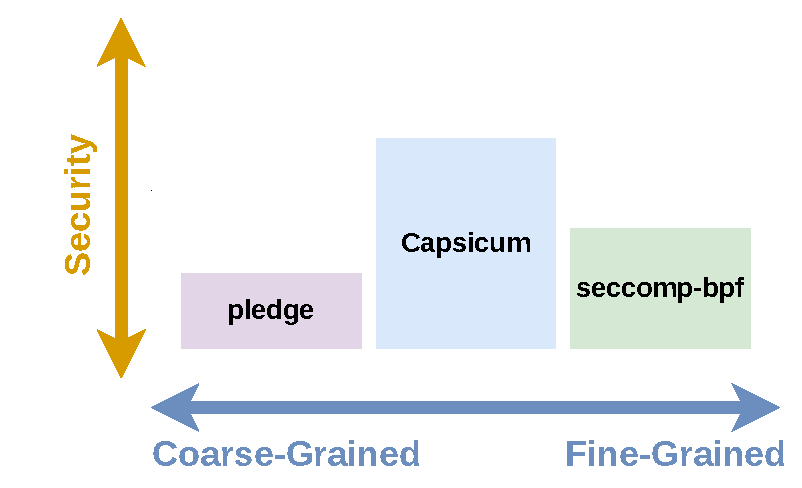
\includegraphics[width=0.8\linewidth]{figs/systemcall-interposition.pdf}
    \caption{Security and granularity trade-offs of pledge,
    Capsicum, and seccomp-bpf.}%
    \label{fig:syscall_interposition}
\end{figure}

In the original Linux seccomp implementation, processes use a special
\texttt{seccomp(2)} system call to enter a secure computing state. By default,
processes that have entered this state are restricted to performing
\texttt{read(2)}, \texttt{write(2)}, \texttt{sigreturn(2)}, and \texttt{exit(2)}
system calls.  Pragmatically, this means that a process could read and write on
its open file descriptors, return from invoked signal handlers, and terminate
itself. All violations of this policy would result in forced termination. In
a 2012 RFC \cite{drewry2012_seccomp_bpf}, Drewry introduced an extension to
seccomp enabling the use of BPF programs\footnote{BPF is a special bytecode
language, originally implemented for packet filtering in BSD Unix
\cite{classic_bpf}. In seccomp-bpf, it was retrofitted for the purpose of
filtering system calls instead.} for the defining filters on system call
arguments. This extension, dubbed seccomp-bpf, enables the creation of
fine-grained seccomp policies that filter on system call numbers and arguments,
providing a high degree of control to applications that wish to sandbox
themselves.

Despite the high degree of control that seccomp-bpf offers to applications, it
has severe usability and security concerns, which make it a poor solution for
ad-hoc confinement by end users. Classic BPF \cite{classic_bpf} is a rather
arcane bytecode language, and writing classic BPF programs by hand is a task
left only to expert users. Further, seccomp-bpf policy is easy to misconfigure,
resulting in potential security violations; for instance, a policy that
specifies restrictions on the \texttt{open(2)} system call but not the
\texttt{openat(2)} system call can be circumvented entirely. Finally, despite
userspace library efforts to abstract away the underlying BPF programs
\cite{libseccomp}, seccomp-bpf remains accessible only to application developers
with significant security expertise.

OpenBSD's pledge \cite{pledge} takes a simpler, coarser-grained approach to
system call filtering than seccomp-bpf, instead grouping system calls into
high-level semantically meaningful categories, such as \texttt{stdio} which
includes \texttt{read(2)} and \texttt{write(2)}, for example
\cite{anderson2017_comparison}. This coarse granularity and simplicity provide
increased usability, but come at the expense of expressiveness. For instance,
there is no canonical way to distinguish subsets of system call groups or filter
system calls by their arguments.  Despite its increased usability for
developers, pledge still suffers from a lack of application transparency just as
seccomp-bpf does, meaning that it is only suitable for use by application
developers rather than end users.

Unlike seccomp-bpf and pledge, which apply filtering rules to system calls
directly, FreeBSD's Capsicum takes the approach of restricting access to global
namespaces via a capability-based implementation \cite{watson2010_capsicum}. In
Capsicum, a process enters \textit{capability mode}  using a special
\texttt{cap\_enter} system call. Once in capability mode, access to global
namespaces is restricted to the capabilities requested by the process, and these
capabilities are inherited across \texttt{fork(2)} and \texttt{execve(2)} calls.
Much like seccomp-bpf and pledge, however, Capsicum is \textit{not} application
transparent, and is designed for use by developers rather than end users.

\paragraph*{Linux Security Modules}
The Linux Security Modules (LSM) API \cite{wright2002_lsm} provides an
extensible security framework for the Linux kernel, allowing for the
implementation of powerful kernelspace security mechanisms that can be chained
together. LSM works by integrating a series of strategically placed
\textit{security hooks} into kernelspace code. These hooks roughly correspond
with boundaries for the modification of kernel objects. Multiple security
implementations can hook into these LSM hooks and provide callbacks that
generate audit logs and make policy decisions.

The LSM API sits at a level of abstraction just above the system call API---a
single LSM hook may cover multiple system calls and a single system call may
contain multiple such LSM hooks. For instance, the \texttt{execve(2)} and
\texttt{execveat(2)} calls both result in a call to the
\texttt{bprm\_set\_creds} and  \texttt{bprm\_committing\_creds} hooks. This
provides a nice level of abstraction compared to system-call-based approaches
like seccomp-bpf \cite{seccomp_bpf, drewry2012_seccomp_bpf} in that a single LSM
hook can cover all closely related security events (recall the issue of
\texttt{open(2)} vs \texttt{openat(2)} in seccomp-bpf).

The Linux kernel ships with a number of LSM-based security modules by default.
Many such modules implement \textit{mandatory access control} (MAC) schemes,
which enable fine-grained access control that can be used to limit the
privileges of \textit{all users}---even the superuser. SELinux
\cite{smalley2001_selinux} and AppArmor \cite{cowan2000_apparmor}, are two such
MAC LSMs, each with its own policy semantics. I discuss each in turn.

SELinux \cite{smalley2001_selinux} was originally developed by the NSA as
a Linux implementation of the Flask \cite{spencer1999_flask} security model.
Under SELinux, system subjects (users, processes, etc.) and system objects
(files, network sockets, etc.) are each assigned corresponding labels. Security
policy is then written based on these labels, specifying the allowed access
patterns between a particular object type and subject type. SELinux's policy
language is famously arcane \cite{schreuders12_towards}, and despite multiple
efforts to introduce automatic policy generation \cite{audit2allow,
macmillan07_madison, macmillan07_madison}, writing and auditing SELinux security
policy remains a task for security experts rather than end users. Further, due
to the difficulty of writing and auditing the complex SELinux policy language,
there is a natural tendency for human policy authors to err on the side of
over-permission, violating the principle of least privilege.

AppArmor (originally called SubDomain) \cite{cowan2000_apparmor} is often touted
as a more usable alternative to SELinux. Rather than basing security policy on
labelling system subjects and objects, AppArmor instead takes the approach of
path-based enforcement.
\todo{continue this}

%\todo{Linux MAC: LSM Hooks, SELinux, AppArmor, TOMOYO, yama}

\subsection{High Level Techniques}
\label{sec:high-level}

In this section, I examine some higher level process confinement techniques that
typically employ more than one of the lower level techniques described in the
previous section (\Cref{sec:low-level}). Although these solutions generally
constitute higher level abstractions, they are not strictly any better than
their lower level counterparts, particularly with respect to the adaptive
process confinement properties outlined in \Cref{sec:introduction}.

\paragraph*{Containerized Package Management}
In Linux, a recent trend of \textit{containerized package management} has
emerged, allowing users to download applications as packages which are then
confined using a combination of lower level techniques exposed by the operating
system. Among the most popular of these containerized package management
frameworks are Docker \cite{docker}, Snap \cite{snap}, and Flatpak
\cite{flatpak}. Typically, a package maintainer or application author would
write a high-level package manifest declaring the privileges required by the
application. This package manifest would then be translated into policy for the
underlying process confinement mechanisms (such as those presented in
\Cref{sec:low-level}). This architecture is depicted in
\Cref{fig:containerized}.

\begin{figure}[htpb]
    \centering
    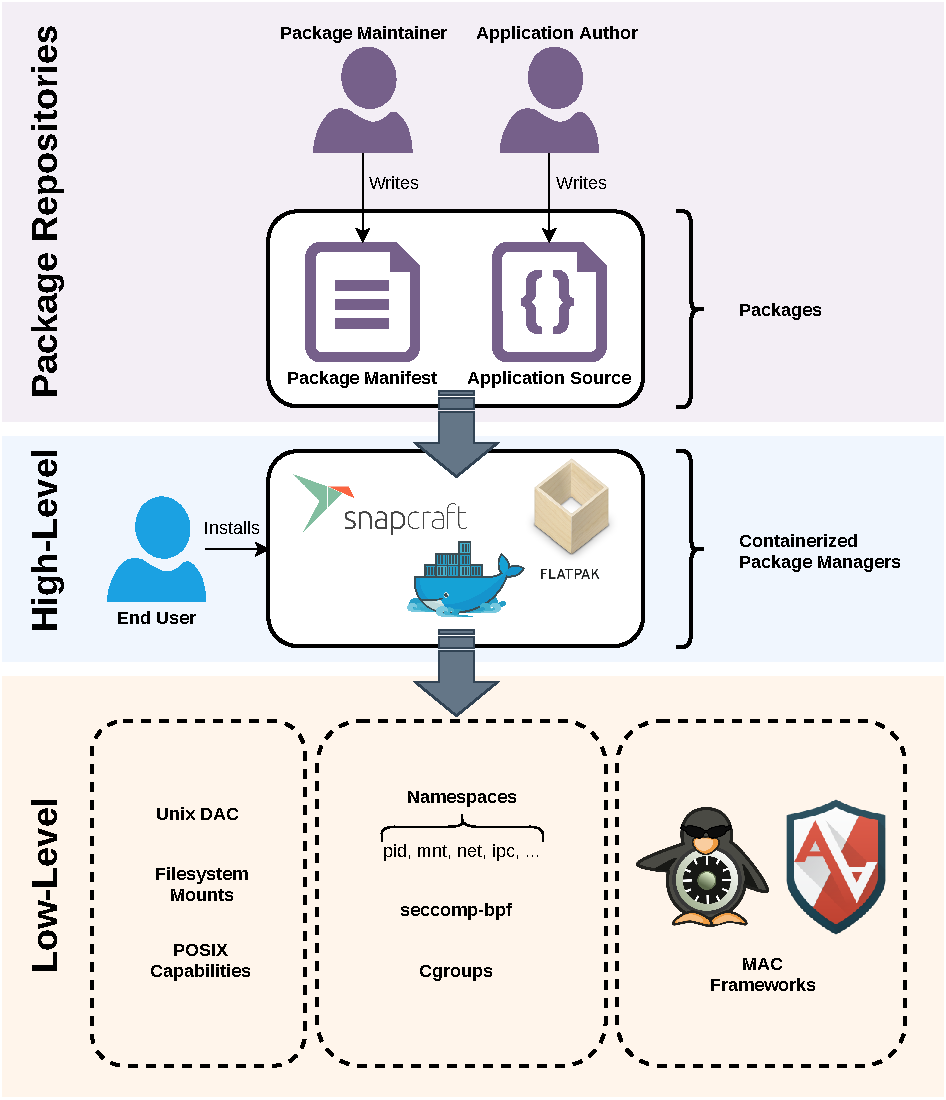
\includegraphics[width=0.9\linewidth]{figs/high-level.pdf}
    \caption{
        The basic architecture of containerized package management solutions for
        Linux, such as Snapcraft \cite{snap}, Flatpak \cite{flatpak}, and Docker
        \cite{docker}. Package maintainers write high-level, coarse-grained
        package manifests, which are then compiled into policy for lower-level
        process confinement mechanisms to enforce.
    }%
    \label{fig:containerized}
\end{figure}

Despite their widespread adoption, these containerized package management
solutions are far from perfect \cite{sultan2019_container_security}. Due to the
coarse granularity of package manifests and high complexity of the underlying
policy enforcement mechanisms, policy for containerized applications tends
toward gross overpermission. Auditability of policy also suffers due to the
disparity between user \textit{expectations} of protection described in package
manifests and the actual policy which is enforced in practice. In effect, five
or six lines of policy in a package manifest may end up generating thousands of
lines of policy across multiple underlying process confinement mechanisms; thus,
auditing the generated policy also becomes a seemingly hopeless task, even for
seasoned security experts.

As a motivating example, consider the package manifest for Snap's Nextcloud\footnote{\url{https://snapcraft.io/nextcloud}}
package, which includes the Apache \texttt{httpd} websever. The package
manifest lists the following permissions for Apache \texttt{httpd}:

\begin{listing}[language=yaml]
confine: strict
/* ... */
apache:
  daemon: simple
  plugs:
  - network
  - network-bind
  - removable-media
\end{listing}

The result, after policy generation, is 411 seccomp-bpf filters and a 653 line
AppArmor policy. The policy is overly permissive, covering a broad scope of
capabilities beyond what would be expected based on the three lines of security
policy defined in the manifest. For instance, the AppArmor profile allows the
execution of over 120 common shell utilities, which is not indicated in the
manifest whatsoever. Further, the policy defined in the generated seccomp-bpf
policy file often does not align with the policy defined in the generated
AppArmor file, adding an extra layer of difficulty to auditing the generated
policy.

Ultimately, the problem with containers as an isolation mechanism lies in the
complexity of the underlying process confinement mechanisms that they leverage.
Namespaces, cgroups, and filesystem mounts are used to virtualize the
containers, while complex mechanisms like seccomp, SELinux, and AppArmor are
used to enforce least privilege. The simplicity of high-level package manifests
belies the complexity underneath, wherein full userlands must be secured for
each application. This can often result in a false sense of security,
particularly when the underlying process confinement mechanisms are
misconfigured, transparently to the end user.

\paragraph*{Confinement with Wrapper Applications}

\todo{Firejail, Bubblewrap, mbox}

\subsection{Summary of Maladaptive Techniques}

\FloatBarrier

% TODO: Maybe move this down ()
\begin{table}
\begin{tabular}{rcccccl}
    \toprule
    Mechanism &
    \rot{\ref{p:1} Robustness} &
    \rot{\ref{p:2} Adoptability} &
    \rot{\ref{p:3} Reconfigurability} &
    \rot{\ref{p:4} Transparency} &
    \rot{\ref{p:5} Usability} &
    Score (max 5) \\
    \midrule
    %Unix DAC            & \emptyc & -       & \halfc  & \halfc  & \halfc  & Maladaptive \\
    POSIX Capabilities   & \emptyc & \halfc  & \halfc  & \halfc  & \emptyc & 1.5         \\
    Namespaces + Cgroups & \halfc  & \halfc  & \emptyc & \emptyc & \emptyc & 1           \\
    ptrace               & \emptyc & \emptyc & \emptyc & \emptyc & \emptyc & 0           \\
    Janus                & \halfc  & \emptyc & \halfc  & \halfc  & \emptyc & 1.5         \\
    seccomp-bpf          & \halfc  & \halfc  & \emptyc & \emptyc & \emptyc & 1           \\
    capsicum             & \halfc  & \halfc  & \emptyc & \emptyc & \emptyc & 1           \\
    pledge               & \emptyc & \halfc  & \emptyc & \emptyc & \emptyc & 0.5         \\
    SELinux              & \emptyc & \emptyc & \emptyc & \emptyc & \emptyc & TODO        \\
    AppArmor             & \emptyc & \emptyc & \emptyc & \emptyc & \emptyc & TODO        \\
    TOMOYO               & \emptyc & \emptyc & \emptyc & \emptyc & \emptyc & TODO        \\
    %Yama                 & \emptyc & \halfc  & \emptyc & \fullc  & \emptyc & 1.5         \\
    %bpfbox              & \emptyc & \emptyc & \emptyc & \emptyc & \emptyc & TODO        \\
    \hline
    Docker               & \emptyc & \halfc  & \emptyc & \halfc  & \halfc  & 1.5         \\
    Snap                 & \emptyc & \halfc  & \emptyc & \halfc  & \halfc  & 1.5         \\
    Flatpak              & \emptyc & \halfc  & \emptyc & \halfc  & \halfc  & 1.5         \\
    Firejail             & \emptyc & \emptyc & \emptyc & \emptyc & \emptyc & TODO        \\
    Bubblewrap           & \emptyc & \emptyc & \emptyc & \emptyc & \emptyc & TODO        \\
    mbox                 & \emptyc & \emptyc & \emptyc & \emptyc & \emptyc & TODO        \\
    \bottomrule
\end{tabular}
\caption{The adaptive evaluation for process confinement techniques discussed in
this section. Since Unix DAC is not a process confinement mechanism in its own
right, it is omitted here. Note that scores for lower level mechanisms \textit{do not}
consider the merits of the higher level mechanisms that make use of them.}
\label{tab:maladaptive}
\end{table}

\section{Semi-Adaptive Process Confinement Approaches}
\label{sec:semi-adaptive}

\subsection{(Semi-)Automated Policy Generation}

\todo{aa\_easyprof, audit2allow, Madison, Polgen}

\todo{systrace}

\todo{Inoue Java policy}

\subsection{(Semi-)Automated Policy Auditing}

\section{Towards Truly Adaptive Process Confinement}
\label{sec:towards}

\subsection{Anomaly Detection Techniques}

\subsection{Extended BPF}

\todo{bpfbox}

\section{Conclusion}
\label{sec:conclusion}


% Uncomment for bibliography:
\nocite{*} % TODO: Comment this out when done
\clearpage
\singlespacing
\printbibliography

\end{document}

% vim:syn=tex
